
This is the fourth in a series of tutorials on the use of the \ajpf\ model checking\index{model checking} program.  This tutorial covers the creation of Java Environments  specifically for use in the verification of Autonomous Systems -- particularly systems that intended to run in some environment, such as the real world, that is not written in Java.

Files for this tutorial can be found in the \texttt{mcapl} distribution in the directory 
\begin{quote}
\texttt{src/examples/verifiableautonomoussystems/chapter5}
\end{quote}
The motorway simulator can be found\index{motorway simulator}
in \texttt{src/examples/motorwaysim}

This tutorials assumes some familiarity \gwendolen\ programming and the creation of environments for multi-agent systems as described \intutorial{\ail}{3}{tutorial:ail:environments}


\section{Where does the Automaton representing a BDI Agent Program Branch?}\index{BDI}\index{program automaton}
\label{sec:branching}

A key part of model-checking is the full exploration of the state\index{model-checking}
space of a program (or model).  It's value is therefore in situations
where there are branching points in the possible execution of a
program.  A program which simply prints out the numbers from 1 to 10,
for instance, needs only to be tested once to see if it actually does
this since there is only one possible execution of the program.  In
general BDI agent programming languages do not implement any\index{BDI}\index{agent programming}
randomness within the language itself so branching in the execution of
a program generally occurs at two points.

Firstly, in a multi-agent system, individual agents may act in\index{multi-agent system!model-checking}
different orders.  Consider two agents, $a_1$ and $a_2$ each with a
simple program which means that $a_1$ does $act_1$ and $a_2$ does
$act_2$.  Then there is potentially a run of this system in which
$act_1$ happens before $act_2$ and another in which $act_2$ happens
before $act_1$.  The \ail-toolkit provides support for different\index{AIL!scheduler}\index{scheduler}
scheduling policies among agents as discussed \intutorial{ail}{3}{tutorial:ail:environments}.  These scheduling policies govern
which agent gets to make a state transition at any one time and can,
for instance, enforce strict turn taking among agents or,
alternatively, select the next agent to make a transition entirely at
random.  Depending upon the policy used then there may be branching
points created in the automata checked by \ajpf.  At present no\index{AJPF!relationship to AIL}
language in \ajpf\ allows two agents to make a transition at exactly
the same time, but this is not in principle excluded.

The second place in which branching may occur is in the information
received by the agent from perception or messages.  Sometimes this\index{perception}\index{message}
information is generated by other agents in the system and so branching
points are caused by the scheduling policy which dictates when agents
perform actions or send messages.  However we may also wish to
represent non-determinism in the environment within which the agents\index{environment!agent}
operate -- for instance we might want to introduce the possibility
that messages get lost.  In that case we can use randomness (as discussed \intutorial{ail}{3}{tutorial:ail:environments}) when we
program our \java\ environment to create such branching.
The \ail-toolkit provides specific support for this randomness in\index{AIL!environment}\index{environment!random}
order both to assist the model-checking process and to allow replay of\index{model-checking!AIL support}
specific paths through a program execution if a bug is detected.

\section{The Problem with Environments}\index{environment!model-checking}
%
This desire to represent non-deterministic behaviour in the agents' environment leads
us to one of the key features of our approach to model-checking autonomous systems.\index{environment!random}\index{model-checking!handling the environment}
When we model check an agent in \ajpf\ (or indeed any model-checking system) we \emph{have to} model check it in the context
of a purely \java\ environment that we have placed it in.  However the reason we may be\index{AJPF!environment}
representing non-determinism in that environment (e.g., message loss) is because we\index{environment!model-checking}
believe that in the `real' environment in which it will actually be deployed different things 
may occur and we wish to understand the effect of this on the system behaviour.

So when model-checking \index{model-checking!handling the environment}
an autonomous hybrid agent system in \ajpf\ we have to construct a \java\ environment that represents a simulation of\index{AJPF!environment}\index{environment!model-checking}
some `real' world.  We can encode assumptions about the behaviour of the
`real' world in this simulation, but we would prefer to minimize such\index{simulation}
assumptions.  For much of our autonomous systems work we try to have
minimal assumptions where the environment asserts or retracts percepts\index{perception}\index{message}
and messages on an entirely random basis.  By this we mean that we do not attempt to model assumptions about the effects an agent's actions may have on the\index{action} world, or assumptions about the sequence in which perceptions may appear to the agent.  This approach is not without its cost in terms of state space and the efficiency of model-checking.  As a result we often do have to build in assumptions about the real world.  An approach to mitigating the potential issues introduced by making assumptions is discussed in~\cite{Ferrando21}.

The process for verifying an agent in this way, is to first analyse
the agent program in order to identify all the perceptions that have\index{verification!agent program}\index{agent programming}
an effect on the program.  In multi-agent systems it is also necessary\index{multi-agent system!model-checking}
to identify all messages that the agent may receive from other agents\index{message}
in the environment.  Once a list of perceptions and messages has been\index{perception}
identified, an environment is constructed for the agent alone in such\index{environment!model-checking}\index{verification environment}
a way that every time the agent takes an action the set of perceptions
and messages available to it are created \emph{at random}.  When model\index{model-checking!handling the environment}
checking, the random selection causes the search tree to branch and
the model checker to explore all environmental possibilities.

We will illustrate this process  with a simple,
but hopefully instructive, example.  There is a fuller discussion of the methodology in~\cite{dennis14:_pract}.


\section{Example: Cars on a Motorway}\index{driverless car!example}\index{cruise control!example}
We explain our approach to model-checking autonomous systems via an\index{model-checking!example}
example of two cars on a motorway\footnote{Examples from this tutorial can be
found in \texttt{src/examples/verifiableautonomoussystems/chapter5}
within the \mcapl\ distribution.  The motorway simulator can be found\index{motorway simulator}
in \texttt{src/examples/motorwaysim}.}

\begin{ourexample}
\label{ex:cruise}
We will consider an intelligent cruise control for a car, focusing simply
on when to accelerate and when to maintain its speed.
The \gwendolen{} code for this is show below.  There are two\index{driverless car!example}\index{cruise control!example}
cars, \lstinline{car1} and \lstinline{car2} and, in both cases, when
the car has a goal to reach the speed limit,
\lstinline{+! at_speed_limit [achieve]}, it accelerates and then
waits until the goal is achieved (The `*' symbol is the \gwendolen{}
syntax for `waiting').  The first car then also sends a message to
car2.  Once the cars have reached the speed limit they perform a
\textbf{\lstinline{maintain_speed}} action followed by a 
\textbf{\lstinline{finished}} action.  Car1 gets the goal to be at 
the speed limit when it perceives that it has started, while Car2 gets
the goal only when it receives a message to achieve the goal.

\begin{lstlisting}[basicstyle=\footnotesize\sffamily,language=Gwendolen,style=easslisting]
:name: car1
                        
:Initial Beliefs:
                                                                                                        
:Initial Goals:
                
:Plans: 
+started: {True} <- +!at_speed_limit[achieve];

+! at_speed_limit [achieve] : {True} <-
        accelerate,
        *at_speed_limit,
        .send(car2, :achieve, at_speed_limit);

+at_speed_limit: {True} <-
        maintain_speed,
        finished;

:name: car2
                        
:Initial Beliefs:
                                                                                                        
:Initial Goals:
                
:Plans: 
+.received(:achieve, G): {True} <- +!G [achieve];

+! at_speed_limit [achieve] : {True} <-
        accelerate,
        *at_speed_limit;

+at_speed_limit: {True} <-
        maintain_speed,
        finished;
\end{lstlisting} 
\label{ex:cars}
\end{ourexample}

\subsection{Executing the Program}
%
In order to execute the above program, it needs to be connected either
to physical vehicles or simulations.  Figure~\ref{fig:motorwaysim}
shows the output in a very simple vehicle simulator.  The simulator
has two cars each in their own motorway lane.  The lanes loop around
so when one car reaches the end of its lane it loops back to the
start.  The simulator reports both the speed of each car and their
distance from the start of the motorway.\index{motorway simulator}

\begin{figure}
\begin{center}
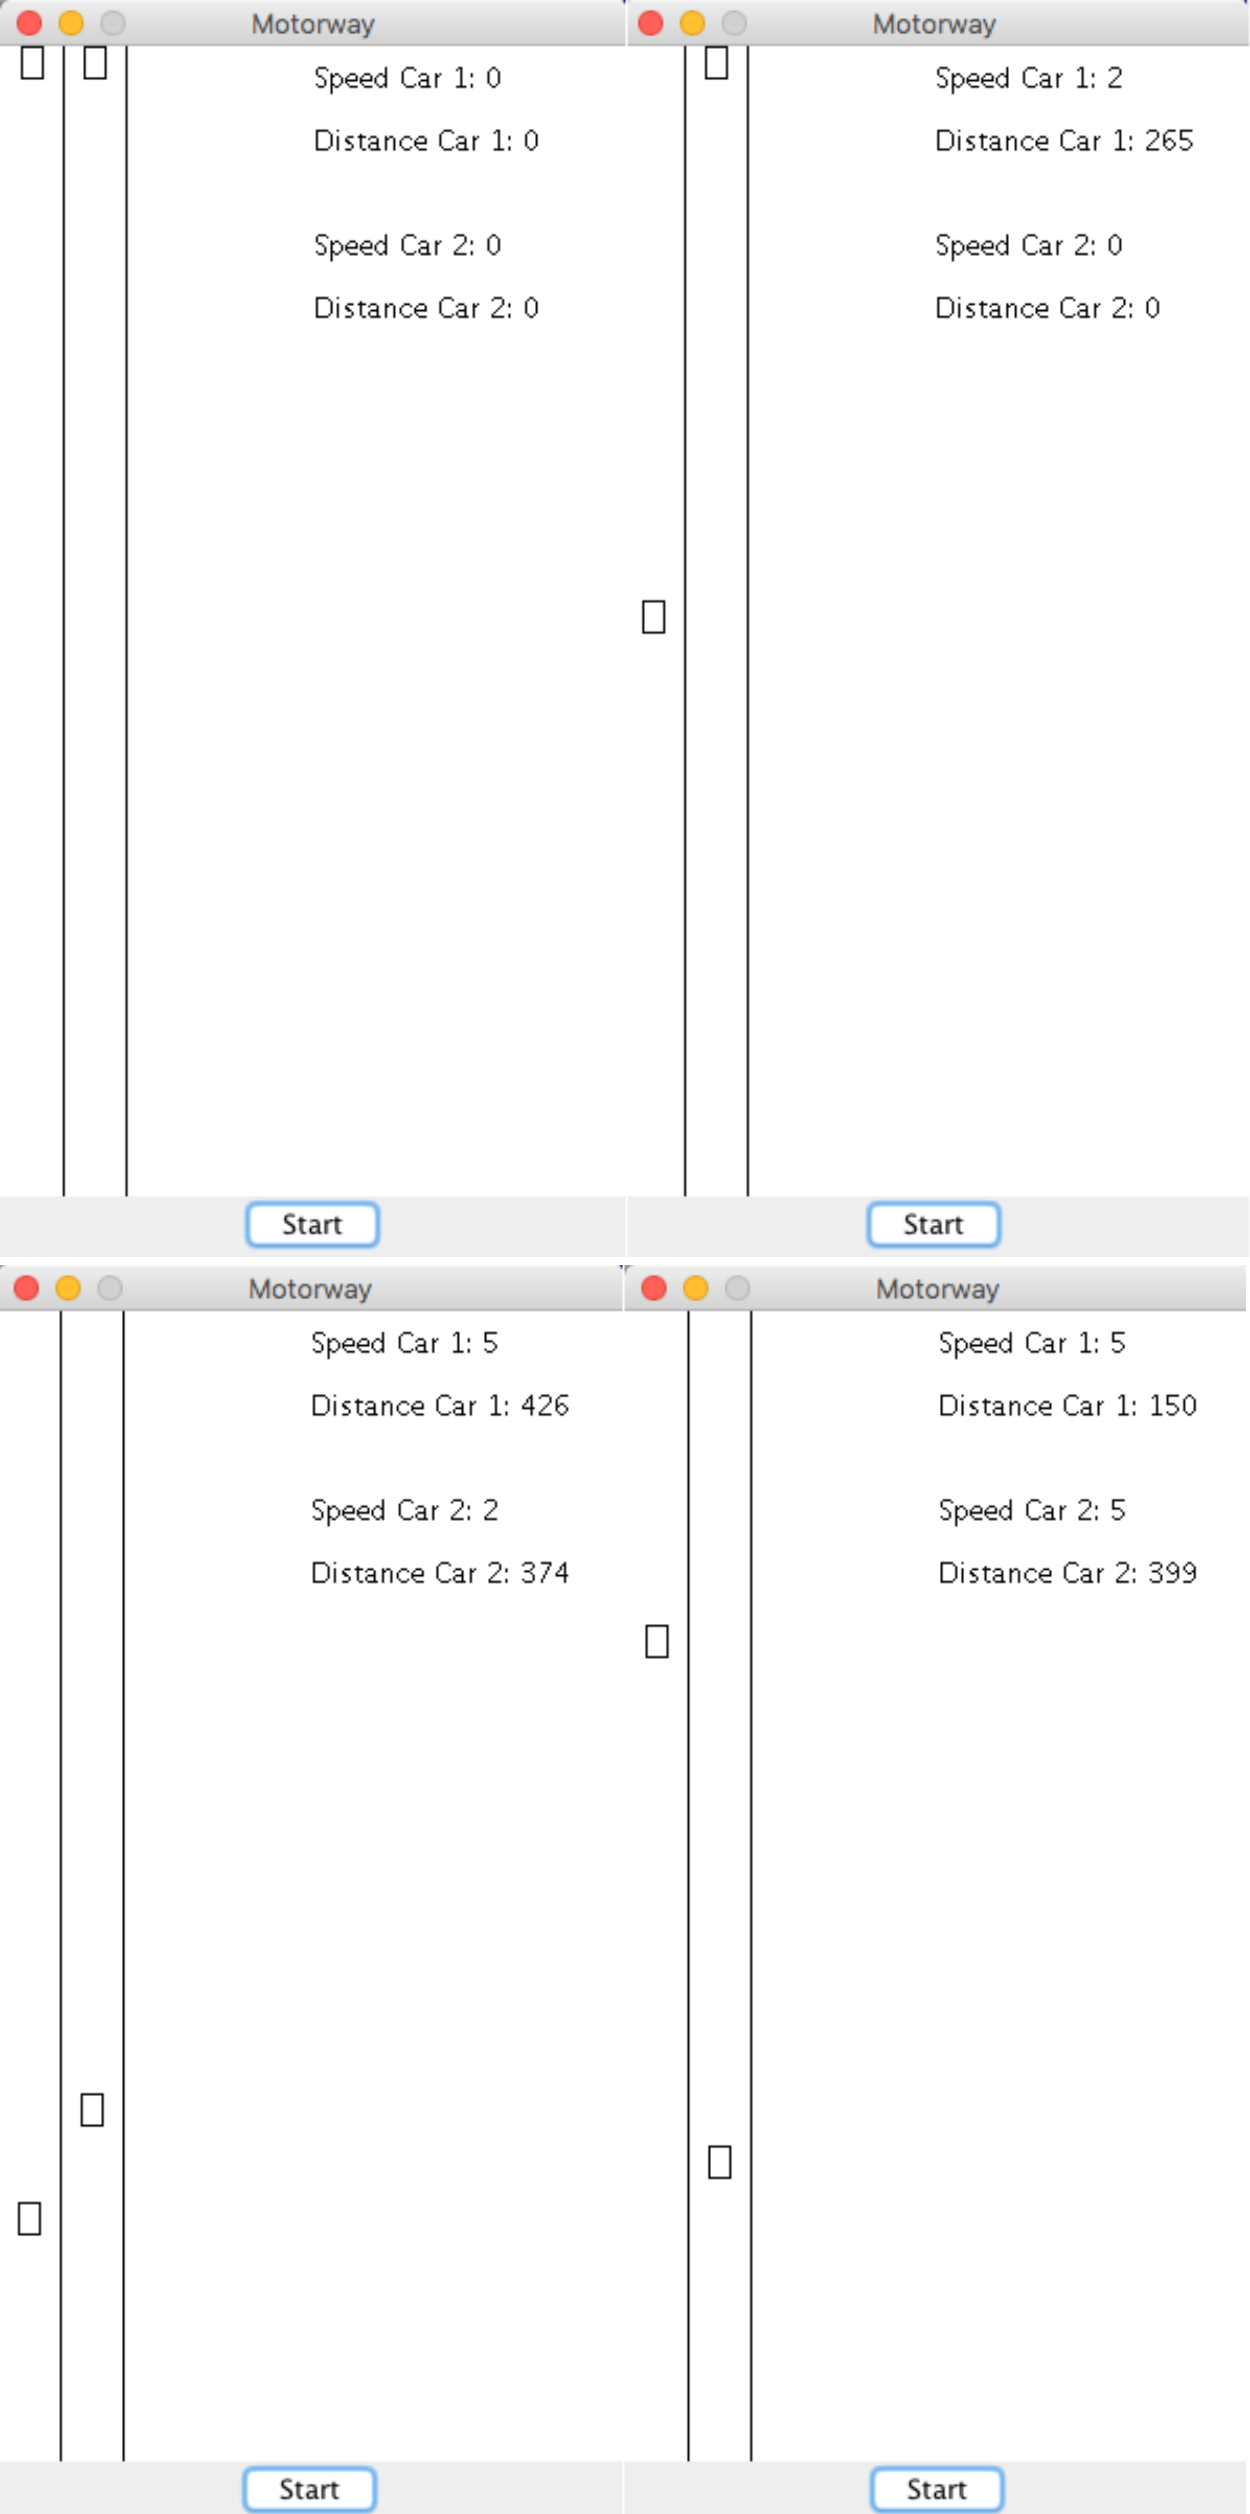
\includegraphics[width=0.6\textwidth]{motorwaysim.png}
\caption{Simulating two cars on a motorway. Images from left to right
  show:\\{} (a) two cars waiting at the start; (b) the first car
  accelerating; (c) as the first car reaches a speed of 5 it messages
  the second car which begins accelerating; until (d) both cars are\index{driverless car!example}\index{message!driverless car example}
  moving at a speed of 5.}\index{cruise control!example}
\label{fig:motorwaysim}
\end{center}
\end{figure}

\begin{sloppypar}
The agents are connected to the simulator via a \java\ environment\index{motorway simulator}
which communicates using a standard socket mechanism.  It reads the
speeds of the cars from the sockets and publishes values for\index{driverless car!example}\index{cruise control!example}
required acceleration to the socket.  If a car's speed becomes larger than 5
then the environment adds a perception that the car is at the speed
limit.  If a car agent performs the \lstinline{accelerate} action\index{action!driverless car example}
then the environment publishes an acceleration of 0.1 to the socket.
If a car agent performs the \lstinline{maintain_speed} action then
the environment publishes an acceleration of 0 to the socket.
\end{sloppypar}

\subsection{Verification: Building a model by Examining the Environment}
%
Suppose we wish to use \ajpf\ to verify our agents for controlling the
two cars.  We cannot include the whole of the motorway simulator
program in our formal verification since it is an external program.
We need to replace the socket calls to this simulator in our \java\
environment with some model of its behaviour.\index{AJPF!environment}\index{driverless car!verification environment}\index{motorway simulator}\index{formal verification}\index{verification environment}\index{cruise control!verification environment}

\begin{sloppypar}
A naive way to set about this might be to capture the obvious
behaviour of the simulator.  We could use a scheduler to alternately
execute a method, generally called \lstinline{do_job} in \ail-supporting environments,  in the simulator to calculate\index{AIL!environment}\index{verification environment}
the position of each car and then to execute one step in the reasoning
cycle of each car.  If a car agent executes \lstinline{accelerate}
then each call of \lstinline{do_job} increases the car's speed by 1.  If
the car agent executes \lstinline{maintain_speed} then the car's speed
remains constant.  As in the \java\ environment that communicated with
the simulator, once the speed has reached 5 this is set as a percept, \lstinline{at_speed_limit},
that the agent can receive.
\end{sloppypar}


Such a model is, in fact, entirely deterministic (like the program that counted to 10 in Section~\ref{sec:branching}) because of the turn
based control of the environment and the two agents.  There is no need for more sophisticated model checking since we can simply run the program once and see what happens.\index{model-checking!handling the environment}

Obviously we can make our model more complex -- for instance we could
introduce a random element into whether the car detects that it has\index{environment!random}\index{verification environment}
reached the speed limit, or exactly how much acceleration is created.
There are some limitations to this, however.  For instance, we need
our model to contain a reasonable number of states, so we can not
simply vary the acceleration by a random double since that would
introduce a very large search space, creating a search branch for each
possible double value that could be used at that point.

Similarly as the world we wish to model becomes more complicated, such
environments inevitably become harder and harder to craft in ways that
behave with appropriate fidelity.

\subsection{Verification: Building a Model by Examining the Agents}
%
The alternative to trying to create a \java\ model to accurately\index{verification environment}
describe the behaviour of the real world is to analyse instead
the inputs in terms of perceptions and messages received by the agent\index{perception}\index{message}
program. This is our approach. We construct a model in which, every
time the agent program queries the environment for perceptions, the
environment returns a random subset of these. In the case
of \lstinline{car1} there are only two perceptions
\lstinline{at_speed_limit} and \lstinline{started} and so we need
an environment that generates inputs from these two.  

The \mcapl\ framework provides support for creating these kinds of environments for \gwendolen\ programs through
an abstract\index{MCAPL Framework}\index{Gwendolen!verification environment}\index{VerificationofAutonomousSystemsEnvironment}
\begin{quote}
\texttt{gwendolen.mas.VerificationofAutonomousSystemsEnvironment}
\end{quote} class that can, in
turn, be sub-classed.  The sub-classes simply have to sub-class the
methods for generating random perceptions, \lstinline{generate_percepts},
and random messages, \lstinline{generate_messages}.\index{perception!verification environment}\index{message!verification environment}

\begin{ourexample}\index{driverless car!verification environment}\index{verification environment}\index{cruise control!verification environment}
%\SetJava
\hspace{0.5cm}
\begin{lstlisting}[basicstyle=\footnotesize\sffamily,language=Gwendolen,style=easslisting]
public Set<Predicate> generate_percepts() 
{
   Set<Predicate> beliefs = new HashSet<Predicate>();
		
   boolean at_speed_limit =
      random_bool_generator.nextBoolean();
   boolean started =
      random_bool_generator.nextBoolean();
   if (at_speed_limit) 
   {
      beliefs.add(new Predicate("at_speed_limit"));
      AJPFLogger.info(logname, "At Speed Limit");
   }
		
   if (started) 
   {
      beliefs.add(new Predicate("started"));
      AJPFLogger.info(logname, "Started");
   }
   return beliefs;
}
\end{lstlisting}
Here, we show the \lstinline{generate_percepts} method.  Two booleans\index{perception!verification environment}
are generated at random and are used to decide whether or not a
percept is added to the set returned to the agent.  For our car example,
the two percepts in question are \lstinline{at_speed_limit}
and \lstinline{started}.  A similar mechanism can be used to generate
messages at random.  A logging mechanism \texttt{AJPFlogger} prints output about the perceptions generated for a user to see.\index{message!verification environment}
\end{ourexample}

\noindent Using this environment many simple properties\index{verification environment}
 are false, for instance \emph{``if car1 accelerates, eventually it will be at the speed
limit''} is false.  This is because the environment does not link the
acceleration action in any way to the car's speed. In fact the actions
taken by the agent in such an environment have no causal link to the
perceptions that are returned. Essentially, we cannot make any
assumptions about whether the software and machinery involved in
making acceleration happen are working, nor whether the sensors for
detecting the car's speed are working.

To prove useful properties with this kind of environment we typically\index{verification environment}
prove properties of the general form
\begin{quote}
\emph{``If whenever the agent does X
eventually the agent believes Y then...''.}
\end{quote}
%  \index{cruise control}
So for instance we can prove, using the above environment, that\index{driverless car!example verification}\index{cruise control!example verification}
``provided that, if car1 invokes acceleration then eventually car1
believes it is at the speed limit, then eventually car1 will invoke
finished'', i.e:
$$\always
(\lactions{car1}{accelerate} \rightarrow \sometime
\lbelief{car1}{at\_speed\_limilt}) \rightarrow \sometime
\lactions{car1}{finished}.
$$ 
%
There are many properties of
this form discussed in the examples in the MCAPL distribution.

Just as we could make our model based on examination of the
environment more complex and so increase the state space, we can\index{environment!model-checking}
reduce the state space for models based on examination of the agents\index{state space}
by linking the generation of percepts to actions.  By default \texttt{VerificationofAutonomousSystemsEnvironment}
\index{perception!verification environment}\index{action!verification environment}\index{VerificationofAutonomousSystemsEnvironment}
 only randomly generates new sets of perception
after an action has been invoked -- any other time the agent polls the environment for perceptions it receives the same set it was sent last time it asked.  While this
does introduce assumptions about the behaviour of the real world --
that changes in perceptions only occur after an agent has taken some
action, it is normally comparatively safe if you can assume that agent
deliberation is very fast compared to the time it takes to execute an
action and for changes in the world to occur.  This reduces the possibilities and the complexity of the
model-checking problem.  \index{model-checking!handling the environment}

It is also possible to make application specific assumptions to constrain the generation of sets by the environment:  for instance that the \lstinline{at_speed_limit} perception can not be included in a set until after the \lstinline{accelerate} action has been performed at least once.  This does increase the risk that the environment used for verification may exclude behaviours that would be observed in the real environment.

